\documentclass[letterpaper,12pt]{article}
\usepackage{booktabs}
\usepackage{bm}
\usepackage{colortbl}
\usepackage{tabularx}
\usepackage{textcomp}
\usepackage{siunitx}
\usepackage{booktabs}
\usepackage{enumitem}
\usepackage{xcolor}
\usepackage{fancyhdr}
\usepackage{caption}
\usepackage{changepage}
\usepackage{amsmath} 
\usepackage{graphicx}
\usepackage{subcaption}
\usepackage[table]{xcolor} 
\usepackage[margin=1in,letterpaper]{geometry} % decreases margins
\usepackage{cite} % takes care of citations
\usepackage[hidelinks]{hyperref} % adds hyper links inside the generated pdf file
% Define the colors
\definecolor{linkcolor}{RGB}{0, 102, 204}
\definecolor{citecolor}{RGB}{34, 139, 34}
\definecolor{urlcolor}{RGB}{255, 69, 0}

% Setup hyperref
\hypersetup{
    colorlinks=false, % colored links
    linkcolor=linkcolor, % color for internal links
    citecolor=citecolor, % color for citations
    urlcolor=urlcolor, % color for URLs
}
\fancypagestyle{logoheader}{
    \fancyhf{}
    \fancyhead[L]{
\includegraphics[width = 3cm]{infn-art-science-universita-degli-studi-di-milano-bicocca-maintainer-universita-studi-milano-bicocca.png}}
    \renewcommand{\headrulewidth}{0pt}
    }
\usepackage{blindtext}
\graphicspath{{immagini/}}
%Required for inserting images
%++++++++++++++++++++++++++++++++++++++++
%Margini 



\begin{document}

\title{{\small Università degli studi Milano-Bicocca  Dipartimento di Fisica - Laboratorio II }\\
    Esperienza Circuiti III}
\author{F. Ballo, S. Franceschina, S. Dolci - Gruppo T1 39}
\date{\today}
\maketitle
\thispagestyle{logoheader}


\begin{abstract}
Nella seguente relazione vengono presentati i risultati ottenuti dalla terza esperienza del corso di Laboratorio II riguardante l'analisi di circuiti elettrici. L'obiettivo di questa esperienza è quello di studiare circuiti RC, RL e RLC in regimi di corrente continua. Imponendo sul circuito, con un generatore di funzioni, un segnale sinusoidale di ampiezza nota, vogliamo ricavare il comportamento del circuito in base alle componenti e in base a dove andiamo a misurare il segnale.
\begin{adjustwidth}{-1cm}{-1cm}
\end{adjustwidth}
\end{abstract}
\tableofcontents
\newpage

\section{Circuiti RC e RL in corrente alternata}

\subsection{Configurazione del circuito e della strumentazione}
Di seguito abbiamo riportato lo schema \ref{fig:config_circuito} utilizzato per riprodurre il circuito in laboratorio con l'utilizzo di una bread-board e degli opportuni componenti. 
\begin{figure}[h!]
    \centering
    \resizebox{0.5\textwidth}{!}{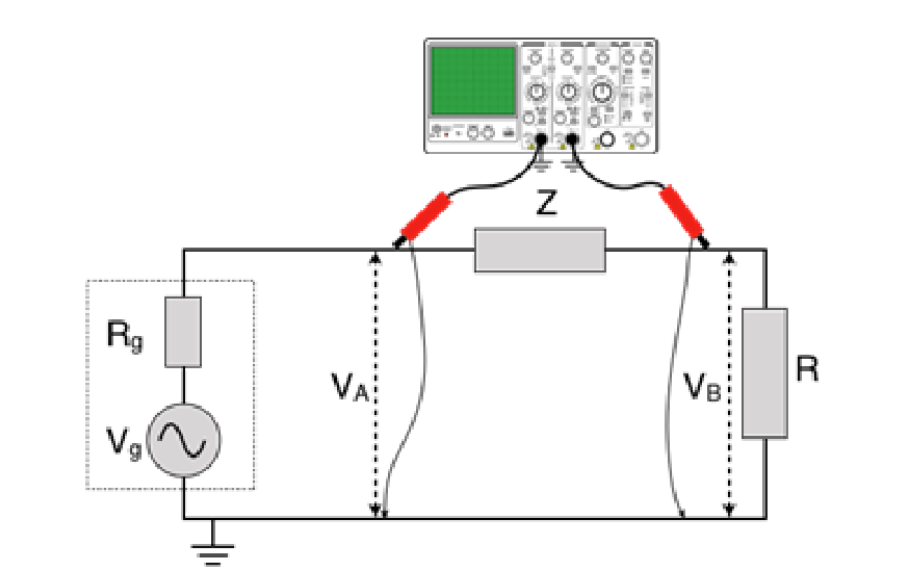
\includegraphics{configurazione circuito.png}}
    \caption{Schema configurazione di circuito, Z rappresenta C o L }
    \label{fig:config_circuito}
\end{figure}
Questa configurazione di circuito rappresenta di fatto un dispositivo a due porte, una di ingresso e uscita, lineare. Per studiare il comportamento di circuiti simili ci si rifà alle funzioni di trasferimento, definite come il rapporto tra il segnale in uscita $V_\text{out}$ e segnale in entrata $V_\text{in}$. 
Tali funzioni dipendono dalla frequenza $H = H(\omega)$ del segnale imposta dal generatore; in particolare si tratta di funzioni complesse: 
$$ H(\omega) = \frac{V_\text{out}(\omega)}{V_\text{in}(\omega)}$$ 
saranno quindi caratterizzate da un modulo e una fase: 
$$ |{H(\omega)| = \frac{|V_\text{out}(\omega)|}{|V_\text{in}(\omega)|}}$$
$$ \phi(\omega) = \phi(\omega)_\text{out} - \phi(\omega)_\text{in} $$
Di seguito riportiamo le funzioni di trasferimento per un circuito RC:

\begin{equation}
\label{eq:Modulo RC}
    |H_C(\omega)| = \frac{R}{\sqrt{R^2 + \frac{1}{\omega^2C^2}}}
\end{equation}

\begin{equation}
    \label{eq:Fase RC}
    \phi = \arctan\left(\frac{1}{R\omega C}\right)
\end{equation}

    
\newpage


\subsection{Dati raccolti RC}
Di seguito riportiamo i dati raccolti per la prima parte dell'esperienza. Dopo aver riprodotto il circuito rappresentato nella figura \ref{fig:config_circuito} abbiamo posizionato le sonde dell'oscilloscopio: sonda 1 per misurare $V_\text{in}$ capacità e sonda 2 per misurare $V_\text{out}$ ai capi della resistenza. Le componenti utilizzate per questo circuito sono:

\begin{enumerate}
    \item Resistenza $R = (100.8\pm0.1)\Omega$
    \item Capacità $C = (99\pm1$) \text{nF}
\end{enumerate}
Successivamente abbiamo misurato al variare della frequenza prodotta dal generatore in un range ():
\begin{enumerate}
    \item Ampiezza del segnale $V_\text{in}$
    \item Ampiezza del segnale $V_\text{out}$
    \item Ampiezza della differenza $V_\text{in} - V_\text{out}$
    \item Differenza di fase tra $V_\text{in} - V_\text{out}$ e $V_\text{in}$
    \item Differenza di fase tra $V_\text{in}$ e $V_\text{out}$
\end{enumerate}



\newpage
\subsection{Analisi dati RC}

\subsubsection{Ai capi della resistenza}

Una volta configurato il circuito, abbiamo variato la frequenza della tensione in ingresso da 200 Hz a 300 MHz seguendo un campionamento logaritmico. Abbiamo misurato la tensione ai capi di R e del generatore con l'oscilloscopio. Tramite la funzione MATH, abbiamo ricavato la differenza tra le due, che rappresenta la tensione ai capi del condensatore. Per ottenere il modulo della funzione di trasferimento abbiamo diviso la tensione ai capi della resistenza per la tensione ai capi del generatore; per ottenere la fase abbiamo misurato tramite lo strumento la differenza di fase fra la tensione in ingresso e la tensione ai capi di R, in seguito abbiamo trasposto le misure in radianti. //
Riportiamo di seguito il grafico del modulo della funzione di trasferimento:

%Figura da inserire

Dato che la teoria prevede 


\subsubsection{Ai capi del condensatore}


\subsection{Conclusioni circuito RC}


\subsection{Dati raccolti RL}
Di seguito riportiamo i dati raccolti per il circuito RL Dopo aver riprodotto lo stesso circuito rappresentato nella figura \ref{fig:config_circuito} cambiano condensatore con induttore abbiamo posizionato le sonde dell'oscilloscopio: sonda 1 per misurare $V_\text{in}$ induttore e sonda 2 per misurare $V_\text{out}$ ai capi della resistenza. Le componenti utilizzate per questo circuito sono:

\begin{enumerate}
    \item Resistenza $R = 1040\ \Omega$
    \item Induttore $L = 0.05\ \text{H}$
\end{enumerate}

Successivamente abbiamo misurato al variare della frequenza prodotta dal generatore in un range ():
\begin{enumerate}
    \item Ampiezza del segnale $V_\text{in}$
    \item Ampiezza del segnale $V_\text{out}$
    \item Ampiezza della differenza $V_\text{in} - V_\text{out}$
    \item Differenza di fase tra $V_\text{in} - V_\text{out}$ e $V_\text{in}$
    \item Differenza di fase tra $V_\text{in}$ e $V_\text{out}$
\end{enumerate}

Le funzioni di trasferimento di un circuito RL sono le seguenti. \\
Ai capi della resistenza:
\begin{equation}
    \label{eq:Modulo RL (resistenza)}
    |H_R(\omega)| = \frac{R}{\sqrt{R^2 + \omega^2L^2}}
\end{equation}

\begin{equation}
    \label{eq:Fase RL (resistenza)}
    \phi_R = \arctan\left(\frac{\omega L}{R}\right)
\end{equation}

E ai capi dell'induttanza:

\begin{equation}
    \label{eq:Modulo RL (induttanza)}
    |H_L(\omega)| = \frac{\omega L}{\sqrt{R^2 + \omega^2L^2}}
\end{equation}

\begin{equation}
    \label{eq:Fase RL (induttanza)}
    \phi_L = \arctan\left(\frac{\omega L}{R}\right)
\end{equation}

\subsection{Analisi dati RL}

\newpage
\subsection{Conclusioni circuito RL}



\newpage
\section{Circuito RLC}

\subsection{Configurazione del circuito}
In questa seconda parte dell'esperimento lo scopo è quello di studiare le funzioni di trasferimento di un circuito RLC in regime di corrente continua.
Di seguito riportiamo le tre funzioni di trasferimento $V_z$ dove z rappresenta tensione su R, L e C:

\begin{enumerate}
    \item \textbf{Traferimento $V_R$} 
    
    $$|H(\omega)| = \frac{R}{\sqrt{R^2 + (\omega L - \frac{1}{\omega C})^2}}$$  
    $$ \phi = \arctan(\frac{\omega^2LC -1 }{\omega CR})$$
    
     \item \textbf{Traferimento $V_C$} 
     
    $$|H(\omega)| = \frac{1}{\sqrt{(1-\omega^2LC)^2 + \omega^2C^2R^2}}$$  
    $$ \phi = \arctan(\frac{\omega CR}{1 - \omega^2 LC})$$
    
     \item \textbf{Traferimento $V_L$} 
     
    $$|H(\omega)| = \frac{\omega^2 L^2}{\sqrt{R^2 + (\omega L - \frac{1}{\omega C})^2}}$$  
    $$ \phi = \arctan(\frac{\omega^2LC -1 }{\omega CR})$$
\end{enumerate}






\begin{figure}[h!]
    \centering
    \resizebox{0.5\textwidth}{!}{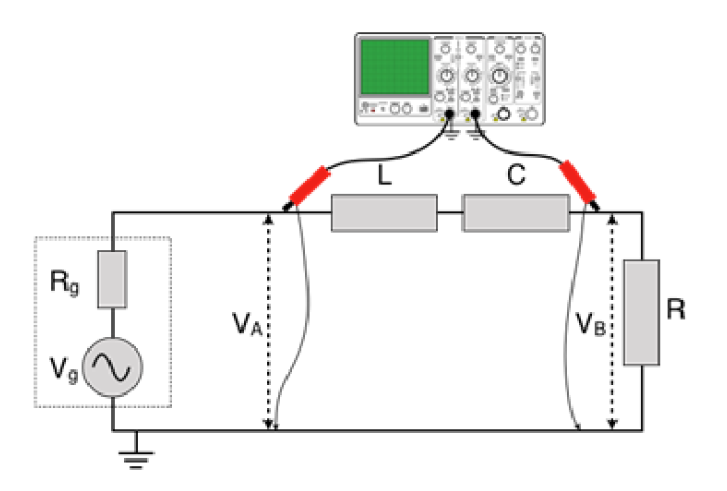
\includegraphics{configRLC.png}}
    \caption{Configurazione circuito RLC}
    \label{fig:configRLC}
\end{figure}



\subsection{Dati raccolti RLC} 
Di seguito riportiamo i dati sulle componenti e la configurazione del circuito studiato:

\newpage
\subsection{Analisi Dati RLC}

\newpage
\subsection{Conclusioni sul circuito RLC}


\newpage
\section{Tabelle misurazioni}



\end{document}
